\documentclass{ctexart}
\usepackage[margin=1in]{geometry}
\usepackage{amsmath}
\usepackage{amssymb}
\usepackage{amsthm}
\usepackage{bm}
\usepackage{hyperref}
\usepackage{graphicx}
\usepackage{caption}
\usepackage{listings}
\usepackage{xcolor}
\usepackage{float}
\usepackage{placeins}
\graphicspath{{figures/}}

% Code style
\lstdefinestyle{code}{
  basicstyle=\ttfamily\small,
  numbers=left,
  numberstyle=\tiny,
  numbersep=8pt,
  keywordstyle=\color{blue},
  commentstyle=\color{teal!70!black},
  stringstyle=\color{orange!70!black},
  showstringspaces=false,
  breaklines=true,
  frame=single,
  framerule=0.3pt,
  rulecolor=\color{black!15}
}
\lstset{style=code}

\title{神经网络基础教程}
\author{}
\date{\today}

\begin{document}
\maketitle
\tableofcontents
\FloatBarrier

\section{人工神经元模型(感知机)}
感知机是人工神经网络中最基本的神经元模型。给定输入向量 $\mathbf{x}=[x_1,\ldots,x_d]^\top$、权重向量 $\mathbf{w}=[w_1,\ldots,w_d]^\top$ 以及偏置 $b$,感知机先计算线性组合,再通过符号函数得到二分类输出:
\begin{equation}
  y = \mathrm{sign}\left(\mathbf{w}^\top \mathbf{x} + b\right),
\end{equation}
其中 $\mathrm{sign}(z)$ 在 $z\ge 0$ 时输出 $1$,否则输出 $-1$。等式 $\mathbf{w}^\top\mathbf{x}+b=0$ 描述的超平面将输入空间划分成两个类别。

\subsection{学习规则}
经典的感知机学习算法在样本 $(\mathbf{x}, t)$($t\in\{-1,1\}$)被误分类时才会更新参数:
\begin{equation}
  \mathbf{w} \leftarrow \mathbf{w} + \eta t \mathbf{x}, \quad b \leftarrow b + \eta t,
\end{equation}
其中 $\eta>0$ 为学习率。该更新会推动决策边界向正确分类方向移动。当数据线性可分时,算法保证在有限步内收敛。

\subsection{几何直观}
图~\ref{fig:perceptron_decision_boundary} 展示了感知机的决策边界以及样本到超平面的符号距离,有助于理解分类几何结构。

\begin{figure}[H]
  \centering
  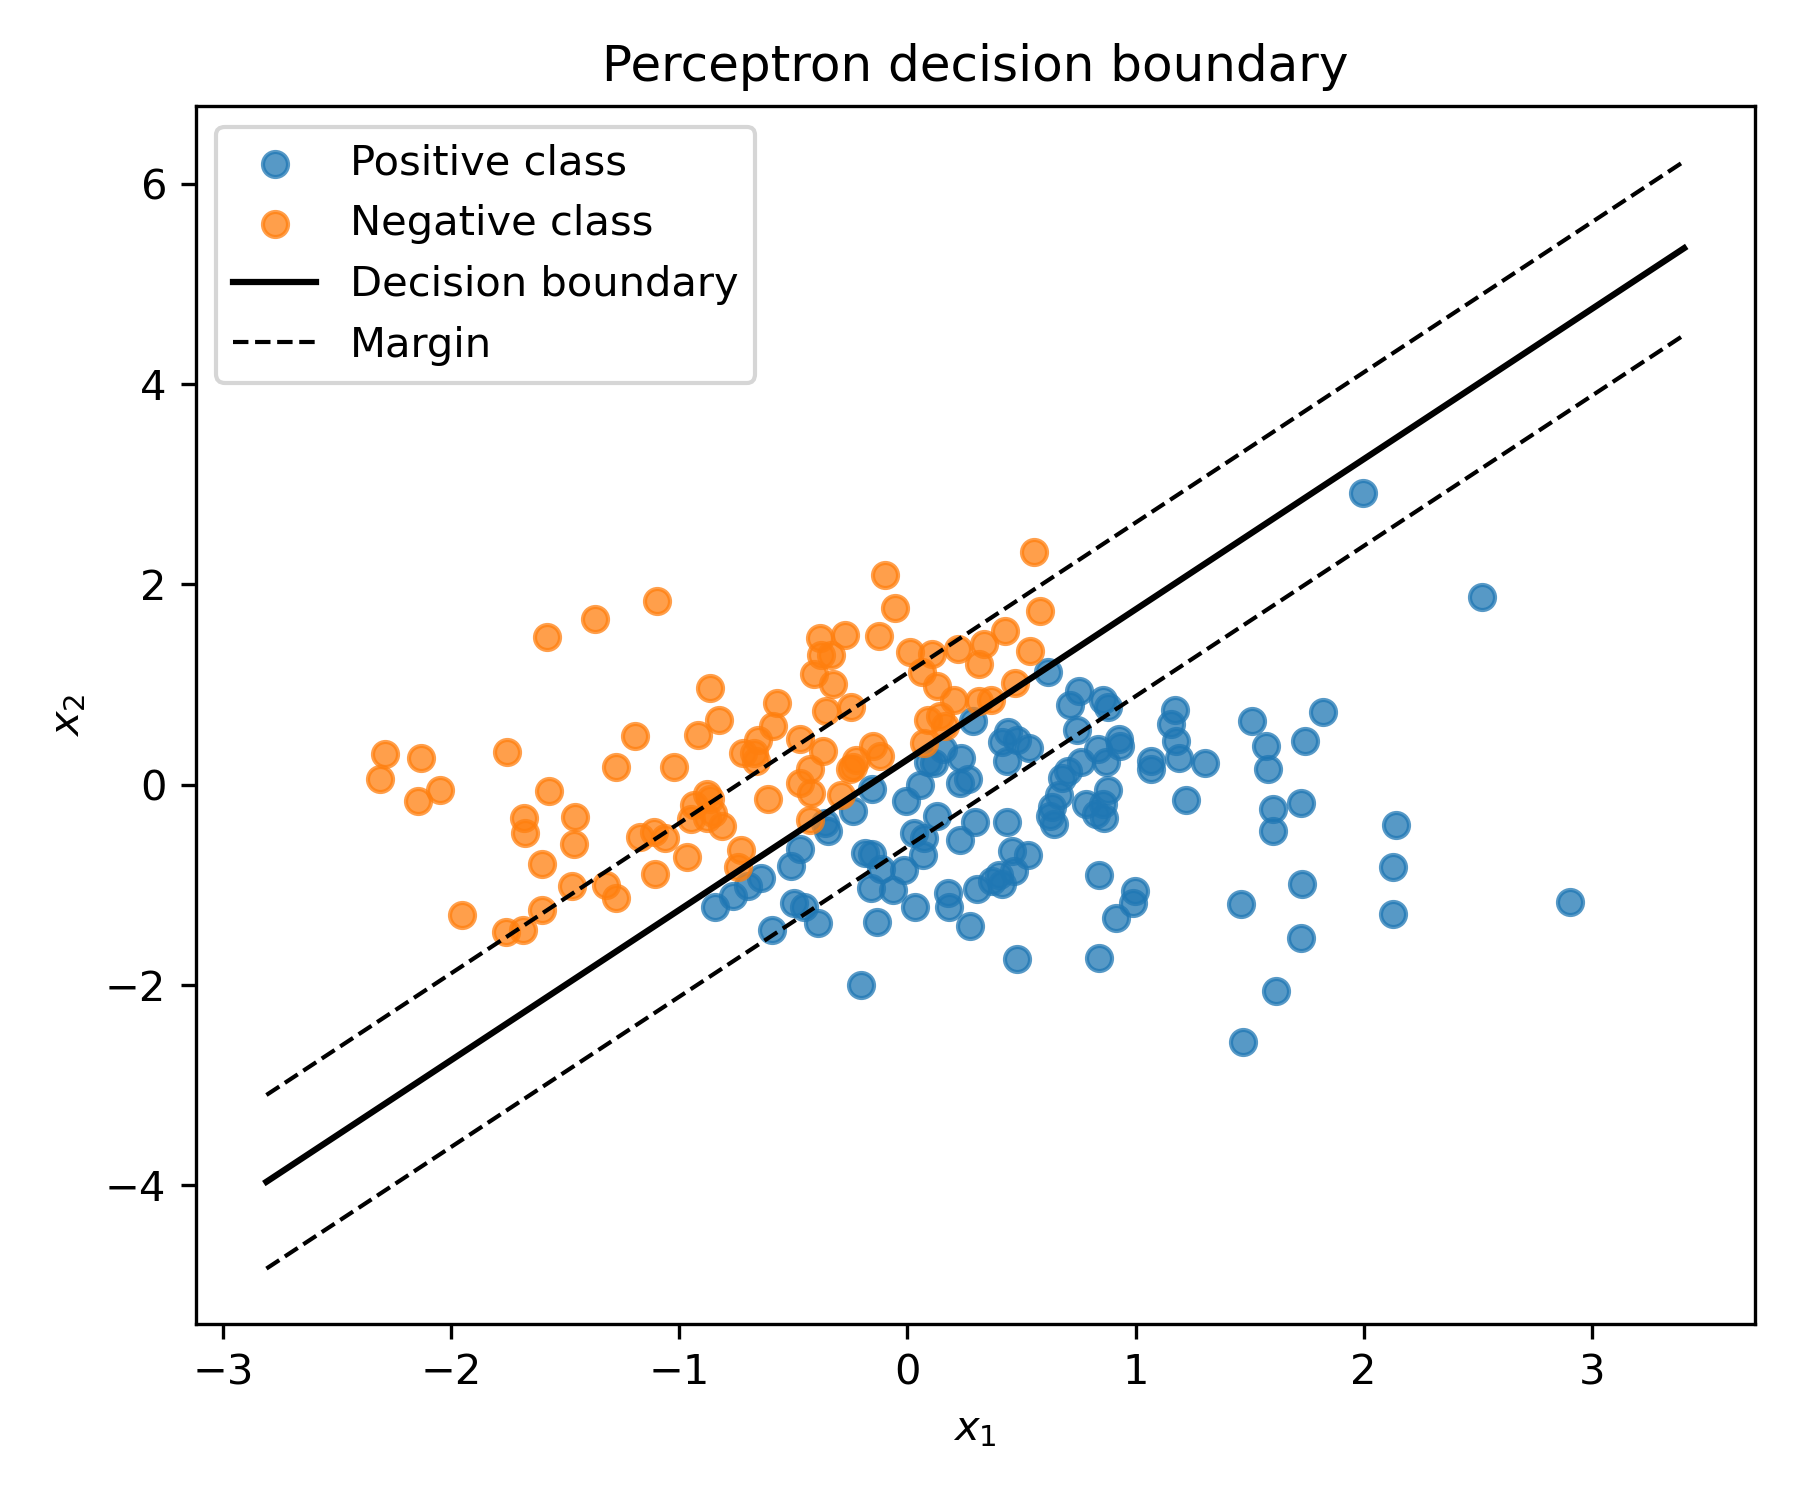
\includegraphics[width=0.7\textwidth]{perceptron_decision_boundary.png}
  \caption{感知机决策边界及其间隔示意。}
  \label{fig:perceptron_decision_boundary}
\end{figure}
\FloatBarrier

\section{多层感知机(MLP)与前向传播}
多层感知机通过堆叠多层神经元并引入非线性激活函数,能够逼近复杂的多维映射。设网络共有 $L$ 层,其前向计算为
\begin{align}
  \mathbf{a}^{(1)} &= \mathbf{W}^{(1)}\mathbf{x} + \mathbf{b}^{(1)}, & \mathbf{h}^{(1)} &= \phi^{(1)}\bigl(\mathbf{a}^{(1)}\bigr), \\
  \mathbf{a}^{(\ell)} &= \mathbf{W}^{(\ell)}\mathbf{h}^{(\ell-1)} + \mathbf{b}^{(\ell)}, & \mathbf{h}^{(\ell)} &= \phi^{(\ell)}\bigl(\mathbf{a}^{(\ell)}\bigr), \\
  \hat{\mathbf{y}} &= \mathbf{h}^{(L)}.
\end{align}
其中 $\phi^{(\ell)}$ 表示第 $\ell$ 层的逐元素激活函数。

\subsection{前向传播算法}
前向传播沿层级顺序依次计算线性变换与非线性映射,以下 Python 代码给出了简洁实现:

\begin{lstlisting}[language=Python, caption={全连接 MLP 的前向传播示例。}]
import numpy as np

def forward_pass(weights, biases, activations, x):
    h = x
    for W, b, act in zip(weights, biases, activations):
        a = W @ h + b
        h = act(a)
    return h
\end{lstlisting}

\subsection{表达能力}
通用逼近定理指出,具有有限神经元的一隐藏层前馈网络在连续激活函数下,可以在紧致域上逼近任意连续函数。更深的网络通过复用中间特征,通常能以更少参数获得同等表示能力。

\begin{figure}[H]
  \centering
  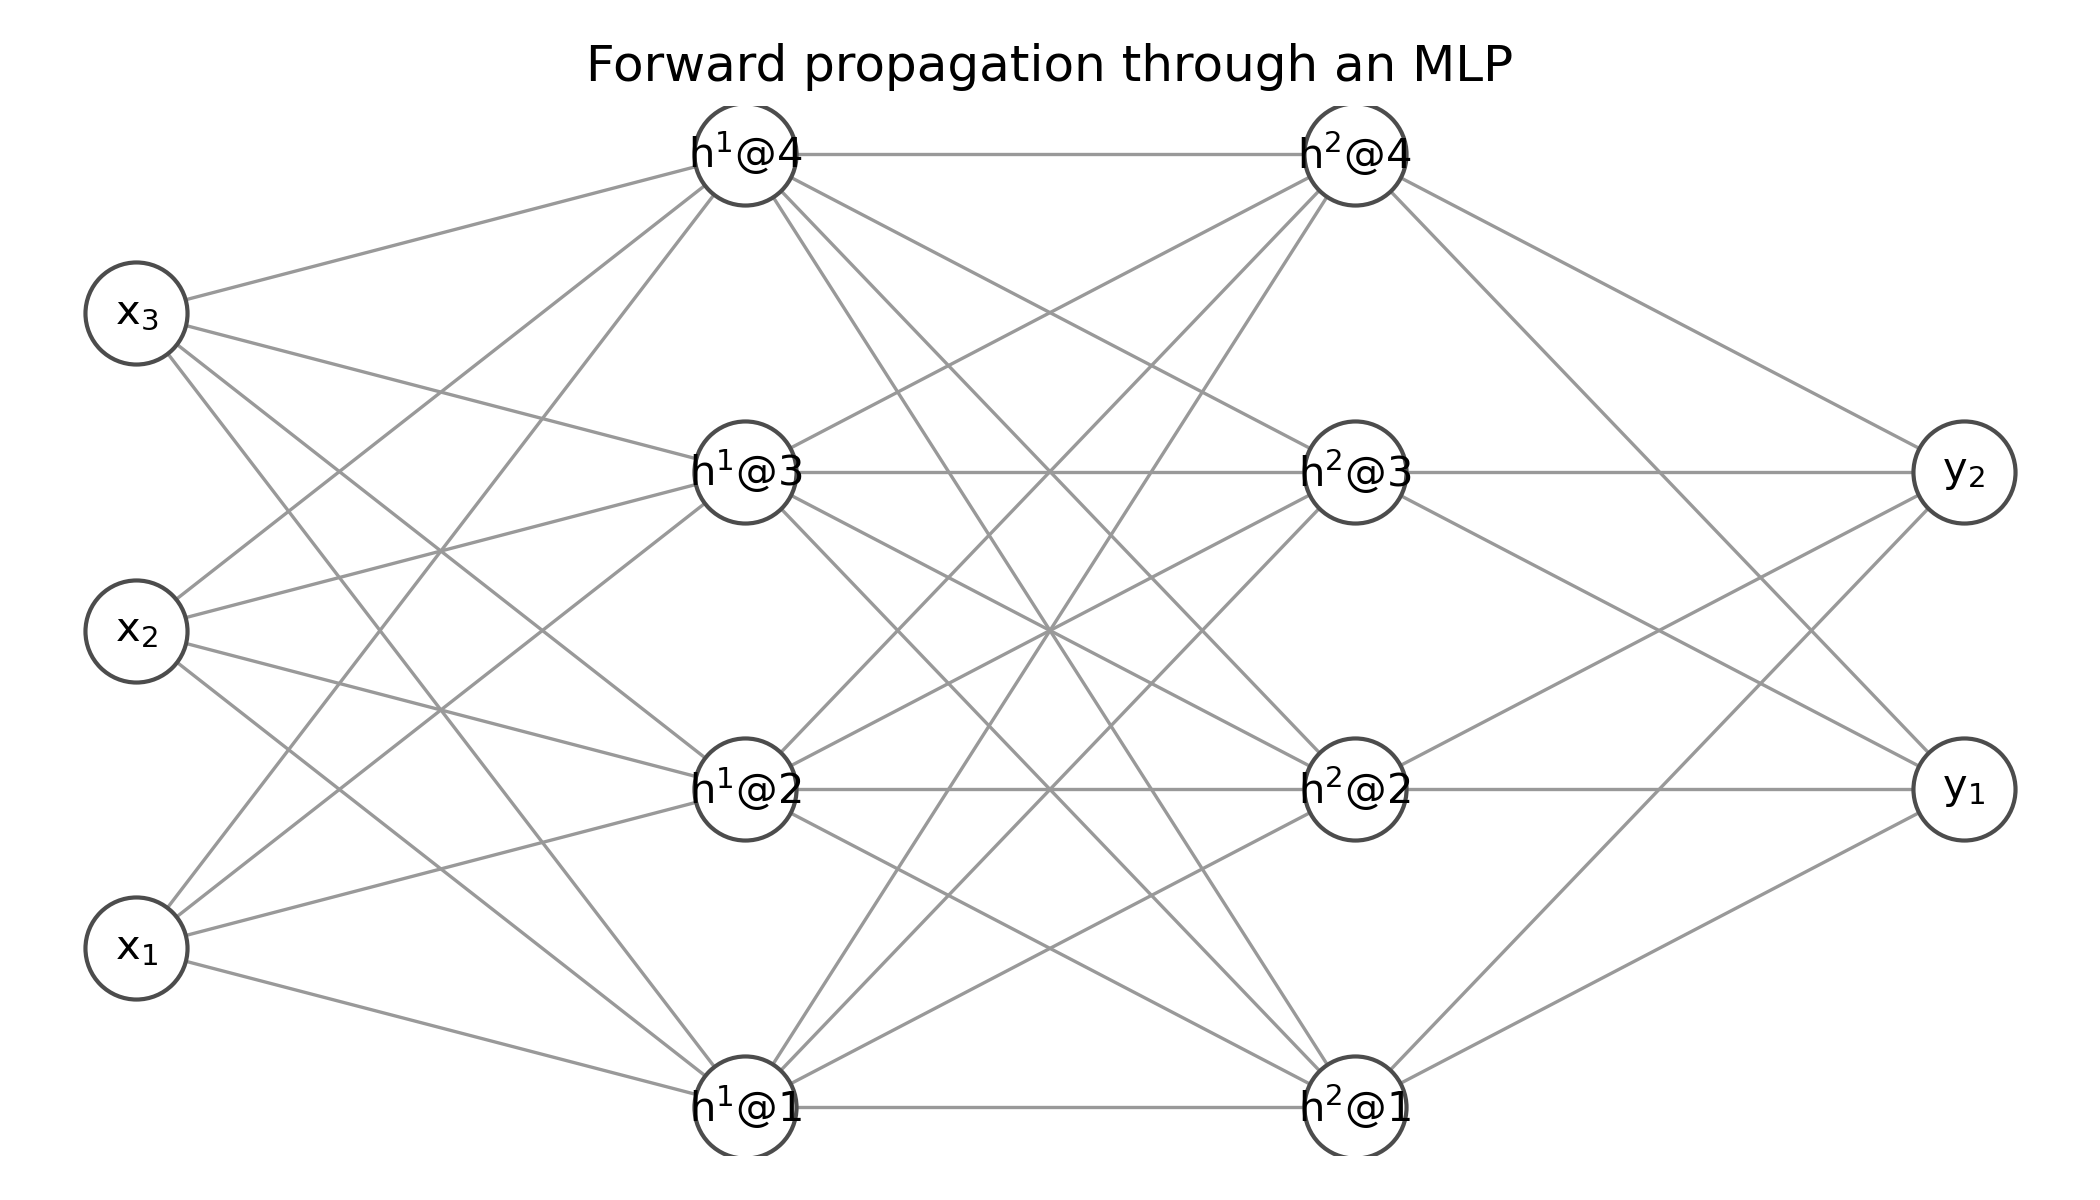
\includegraphics[width=0.8\textwidth]{mlp_forward_pass.png}
  \caption{MLP 的前向传播流程,线性变换与非线性激活交替进行。}
  \label{fig:mlp_forward_pass}
\end{figure}
\FloatBarrier

\section{激活函数}
激活函数为网络提供非线性能力,也影响梯度传播特性。图~\ref{fig:activation_functions} 比较了常见激活函数的曲线形状。

\subsection{Sigmoid}
Logistic Sigmoid 将实数压缩到 $\left(0,1\right)$:
\begin{equation}
  \sigma(z) = \frac{1}{1 + e^{-z}}, \quad \sigma'(z) = \sigma(z)\bigl(1-\sigma(z)\bigr).
\end{equation}
Sigmoid 在 $|z|$ 大时趋于饱和,可能导致梯度消失。

\subsection{Tanh}
双曲正切函数为零中心分布:
\begin{equation}
  \tanh(z) = \frac{e^{z} - e^{-z}}{e^{z} + e^{-z}}, \quad \frac{d}{dz}\tanh(z) = 1 - \tanh^2(z).
\end{equation}
相较 Sigmoid,其输出范围扩大至 $(-1,1)$,更利于梯度传播。

\subsection{ReLU}
修正线性单元定义为
\begin{equation}
  \mathrm{ReLU}(z) = \max(0, z), \quad \mathrm{ReLU}'(z) = \begin{cases}1,& z>0,\\0,& z<0.\end{cases}
\end{equation}
ReLU 易于优化,但若神经元长期处于负半轴,会出现 ``死亡 ReLU'' 问题。

\subsection{Leaky ReLU}
Leaky ReLU 在负半轴保留小斜率以缓解死亡问题:
\begin{equation}
  \mathrm{LeakyReLU}(z) = \begin{cases} z,& z \ge 0,\\ \alpha z,& z < 0,\end{cases}
\end{equation}
常取 $\alpha \approx 0.01$。

\subsection{GELU}
GELU 使用高斯累积分布函数对输入加权:
\begin{equation}
  \mathrm{GELU}(z) = z \Phi(z) = \frac{z}{2}\left[1 + \mathrm{erf}\left(\frac{z}{\sqrt{2}}\right)\right],
\end{equation}
其中 $\Phi$ 是标准正态分布的累积分布函数,$\mathrm{erf}$ 为误差函数。GELU 的平滑性质在 Transformer 中表现突出。

\begin{figure}[H]
  \centering
  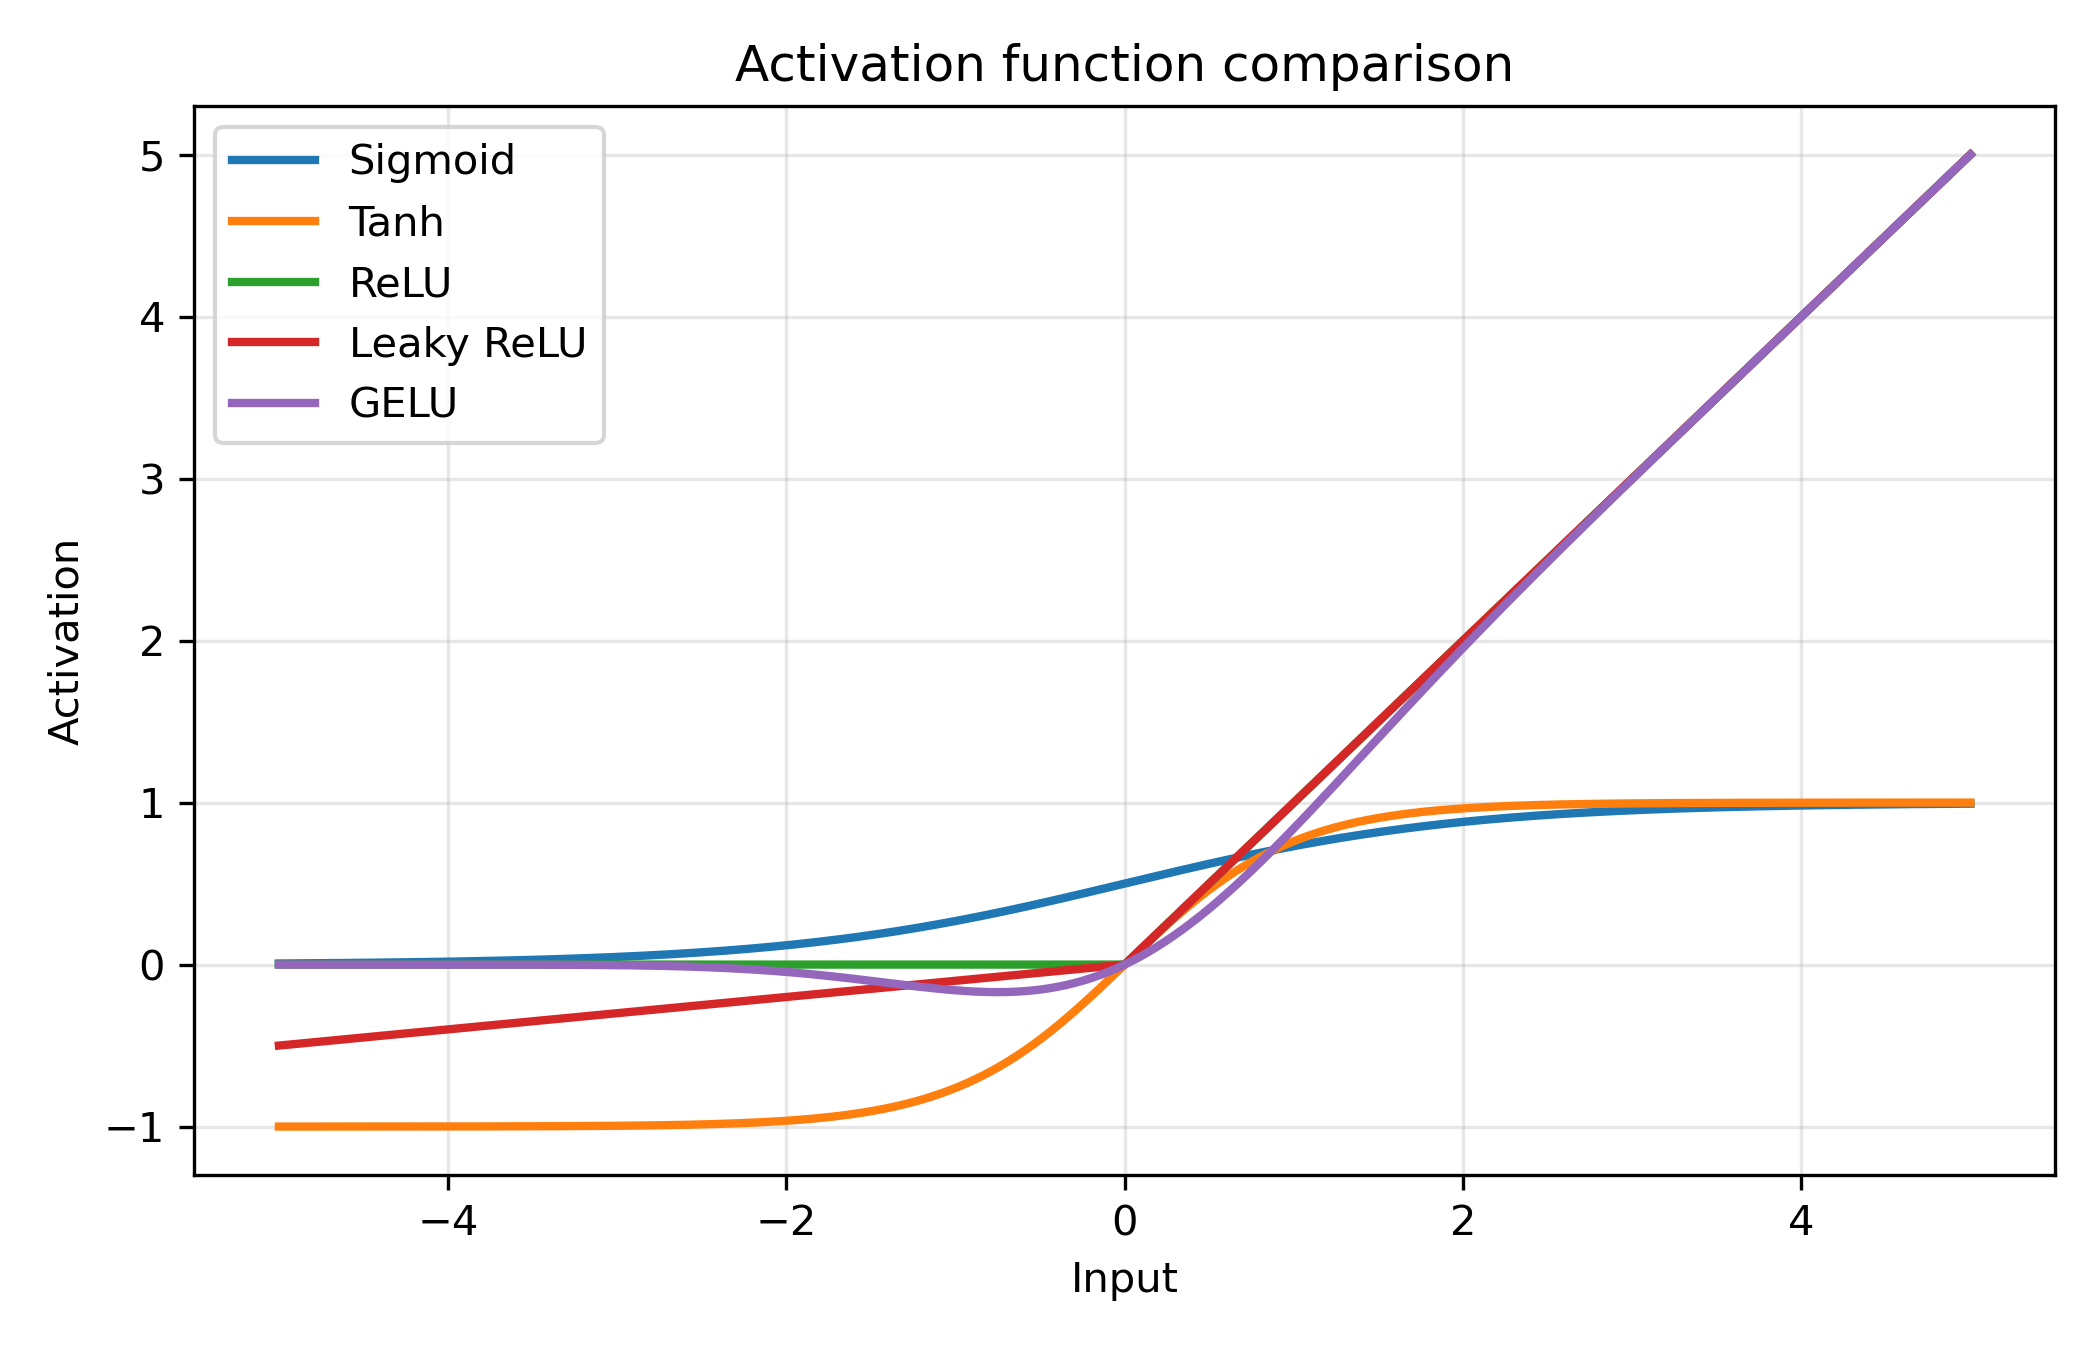
\includegraphics[width=0.8\textwidth]{activation_functions.png}
  \caption{常见激活函数曲线对比。}
  \label{fig:activation_functions}
\end{figure}
\FloatBarrier

\section{损失函数}
损失函数衡量模型预测与真实标签之间的差异,是梯度驱动优化的目标。

\subsection{均方误差(MSE)}
对于回归任务,目标 $t_i$ 与预测 $\hat{y}_i$ 的均方误差为
\begin{equation}
  \mathcal{L}_{\mathrm{MSE}} = \frac{1}{N} \sum_{i=1}^{N} \bigl(\hat{y}_i - t_i\bigr)^2,
\end{equation}
其关于 $\hat{y}_i$ 的梯度为 $\frac{2}{N}(\hat{y}_i - t_i)$。

\subsection{交叉熵}
二分类的交叉熵损失使用概率输出 $p_i$:
\begin{equation}
  \mathcal{L}_{\mathrm{BCE}} = -\frac{1}{N} \sum_{i=1}^{N} \left[t_i \log p_i + (1-t_i) \log(1-p_i)\right].
\end{equation}
对于多分类问题,若 softmax 输出为 $p_{i,k}$,目标 $t_{i,k}$ 为 one-hot 编码,则
\begin{equation}
  \mathcal{L}_{\mathrm{CE}} = -\frac{1}{N} \sum_{i=1}^{N} \sum_{k=1}^{K} t_{i,k} \log p_{i,k}.
\end{equation}

\subsection{Huber 损失}
Huber 损失兼具 L1 与 L2 的优点,对异常值更稳健:
\begin{equation}
  \mathcal{L}_{\delta}(r) = \begin{cases}
    \tfrac{1}{2} r^2, & |r| \le \delta, \\
    \delta(|r| - \tfrac{1}{2}\delta), & |r| > \delta,
  \end{cases}
\end{equation}
其中 $r = \hat{y} - t$,$\delta$ 控制 L2 与 L1 的切换位置。

\begin{figure}[H]
  \centering
  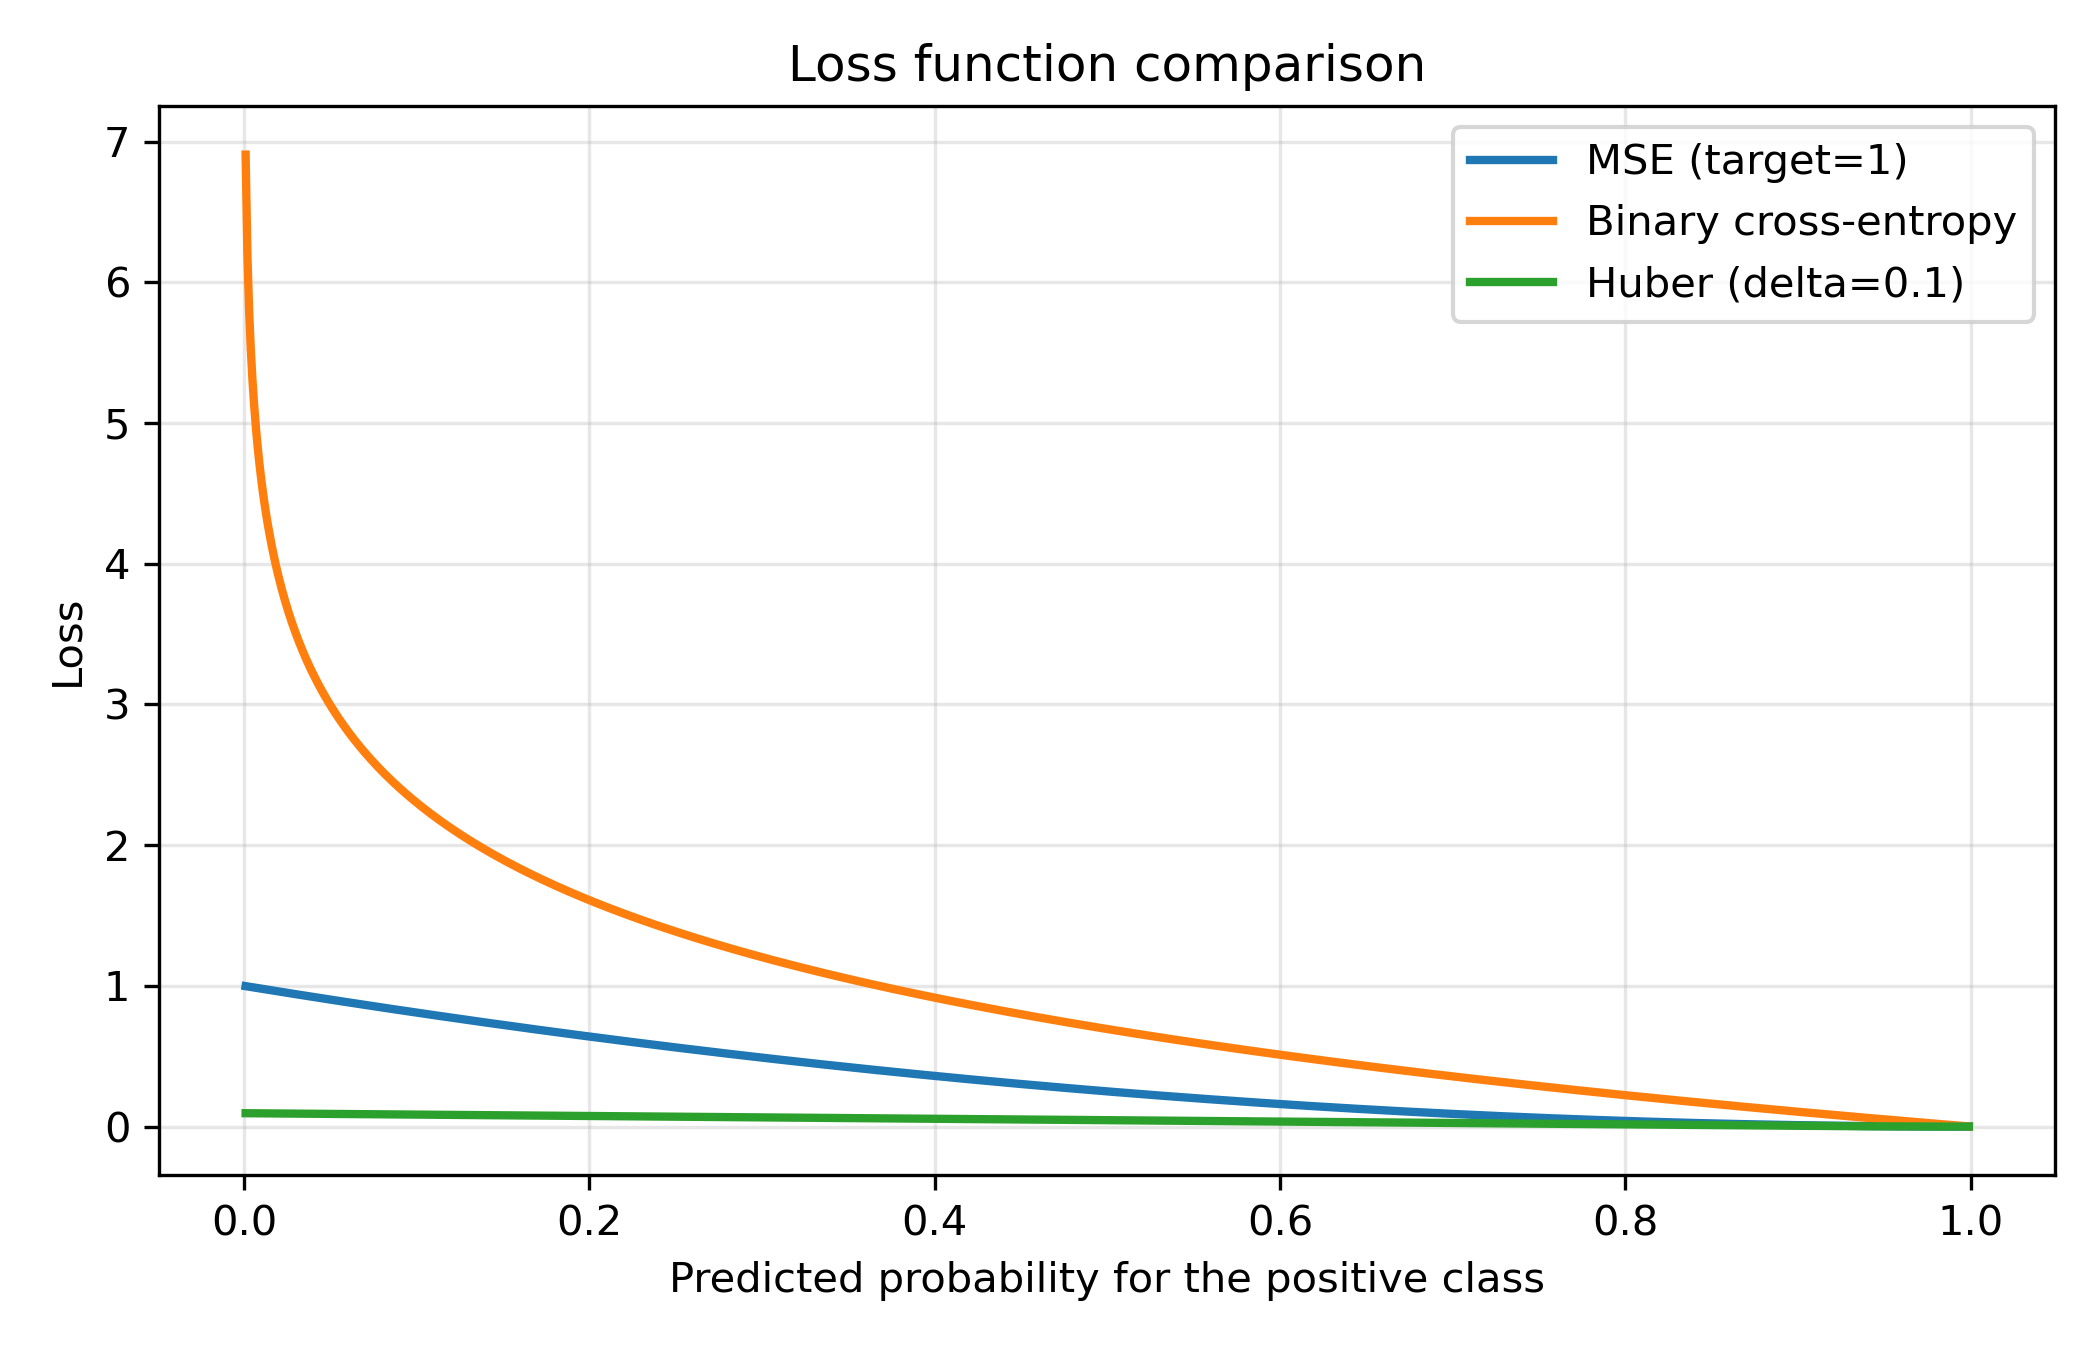
\includegraphics[width=0.8\textwidth]{loss_functions.png}
  \caption{MSE、二元交叉熵及 Huber 损失的曲线形状比较。}
  \label{fig:loss_functions}
\end{figure}
\FloatBarrier

\section{实践建议}
\begin{itemize}
  \item \textbf{参数初始化:} 使用 Xavier 或 He 初始化可避免激活值爆炸或消失。
  \item \textbf{归一化:} 批归一化或层归一化帮助稳定不同层的分布。
  \item \textbf{优化方法:} Adam、RMSprop 等自适应算法能动态调整学习率。
  \item \textbf{正则化:} Dropout、权重衰减、提前停止等方法可缓解过拟合。
\end{itemize}

\end{document}
